
\documentclass[12pt,a4paper,twoside]{book}

%% general usepackage stuff
\usepackage{times}
\usepackage{mathptmx}
\usepackage{amsmath}
\usepackage{booktabs}
\usepackage{graphicx}
\usepackage{titlesec}
\usepackage{amssymb}
\usepackage[utf8]{inputenc}
\usepackage[ngerman]{babel}

\usepackage{color}

%% labels and page stuff
\renewcommand{\labelitemi}{$\diamond$}
\renewcommand{\labelitemii}{$\circ$}

\setcounter{secnumdepth}{3}

%\setlength{\oddsidemargin}{-0.5cm}
%\setlength{\evensidemargin}{-0.5cm}

\setlength{\oddsidemargin}{4.58mm}%final
\setlength{\evensidemargin}{-4.92mm}%final


\setlength{\textwidth}{15.95cm}%final
\setlength{\textheight}{23.5cm}
\setlength{\voffset}{-1.45cm} %


%% todo
\newcommand{\todo}[1]{\textcolor{red}{[todo: }#1\textcolor{red}{]}}
\newcommand{\todoh}[1]{} 
\newcommand{\done}[1]{} 

%% smallerText
\newcommand{\smallerTextSize}{10}
\newcommand{\smallerTextSkip}{12}
\newcommand{\smallerBegin}{\fontsize{\smallerTextSize}{\smallerTextSkip}\selectfont}
\newcommand{\smallerEnd}{\normalsize}
\newcommand{\smaller}[1]{\smallerBegin #1\smallerEnd}

%%reference to defintion
\newcommand{\defref}[1]{\ref{#1} on page \pageref{#1}}

%% special, short for shell
\newcommand{\shl}[1]{\sf \small #1\rm\normalsize}

%% indentation in tables
\newcommand{\tabind}[1]{\rule{#1mm}{0cm}}

%% smaller in captions
\newcommand{\captionfonts}{\smallerBegin}
                                                                                                                                                                              
\makeatletter  % Allow the use of @ in command names
\long\def\@makecaption#1#2{%
  \vskip\abovecaptionskip
  \sbox\@tempboxa{{\captionfonts #1: #2}}%
  \ifdim \wd\@tempboxa >\hsize
    {\captionfonts #1: #2\par}
  \else
    \hbox to\hsize{\hfil\box\@tempboxa\hfil}%
  \fi
  \vskip\belowcaptionskip}
\makeatother   % Cancel the effect of \makeatletter

%% clear page before new chapter
\makeatletter
\def\cleardoublepage{\clearpage\if@twoside \ifodd\c@page\else
\hbox{}
\vspace*{\fill}
\begin{center}
%This page intentionally contains only this sentence.
\end{center}
\vspace{\fill}
\thispagestyle{empty}
\newpage
\if@twocolumn\hbox{}\newpage\fi\fi\fi}
\makeatother

%% abbreviations
\usepackage{nomencl}
\let\abbrev\nomenclature
\renewcommand{\nomname}{List of Abbreviations}
\setlength{\nomlabelwidth}{.25\hsize}
\renewcommand{\nomlabel}[1]{#1 \dotfill}
\setlength{\nomitemsep}{-\parsep}
\makenomenclature
\newcommand{\Listofabbrev}{
\printnomenclature
\newpage
}

%% chapter title formatting
\titleformat{\chapter}[display]{ \raggedleft }{\fontsize{52}{63}\selectfont \bf \thechapter }{0.2cm}{\fontsize{32}{38.7}\selectfont  }[]

%% haeder formatting
\renewcommand{\chaptermark}[1]{%
\markboth{\chaptername
\ \thechapter.\ #1}{}}
\renewcommand{\sectionmark}[1]{\markright{\thesection.\ #1}}
\usepackage{fancyhdr}
\pagestyle{fancy}
\fancyhf[LEH,ROH]{\thepage}
\fancyhf[REH]{\smaller{\nouppercase{\leftmark}}}
\fancyhf[LOH]{\smaller{\it \nouppercase{\rightmark}}}
\fancyhf[COF]{\rule{0.2cm}{0.0cm}}
\fancyhf[CEF]{\rule{0.2cm}{0.0cm}}
\renewcommand{\headrulewidth}{0pt}

%% macro for res
%\usepackage{svg}
%\usepackage{amsmath}
%\newcommand{\printlabel}{}
%\newcommand{\abcdef}[1]{\tiny #1 \normalsize}

		%% arguments: graphics file, label, caption, smallcaption
\newcommand{\insertFigure}[4]{\begin{figure}[top] \smallerBegin \centering \includegraphics{#1}  \\  \caption{\label{#2}\smallerBegin #3 \footnotesize{#4}  \smallerEnd }  
\end{figure}	}
%% macro for figures with short caption
		%% arguments: graphics file, label, caption, smallcaption, shortcaption
\newcommand{\insertFigureShort}[5]{\begin{figure}[top] \smallerBegin \centering \includegraphics{#1} \label{#2} \\ \caption[#5]{\smallerBegin #3 \footnotesize{#4} \smallerEnd } 
\end{figure}	}
%\renewcommand{\topfraction}{1}

\newcommand{\spaceafterpar}{\vspace{14.48pt}}

\renewcommand{\floatpagefraction}{.75} % vorher: .5
\renewcommand{\textfraction}{.1}       % vorher: .2
\renewcommand{\topfraction}{.8}        % vorher: .7
\renewcommand{\bottomfraction}{.5} 
\setcounter{topnumber}{3}              % vorher: 2
\setcounter{bottomnumber}{2}           % vorher: 1
\setcounter{totalnumber}{5}            % vorher: 3
%from: http://www.matthiaspospiech.de/latex/vorlagen/allgemein/preambel/9/

%macros for tables
    %% arguments: columns
\newcommand{\tableBegin}[1]{\begin{table}[top] \begin{center} \smallerBegin \begin{tabular}{#1}}
		%% arguemtns: caption, label
\newcommand{\tableEnd}[2]{ \end{tabular} \smallerEnd \end{center} \caption{#1} \label{#2}	\end{table}}

%% shortcuts
\newcommand{\emit}[1]{\item \emph{#1}:}
\newcommand{\firstappear}[2]{\emph{#1} (#2) \abbrev{#2}{#1}}

\hyphenation{or-gan-izing}

%% definitions

\newtheorem{definition}{Definition}

%% examples
\newcommand{\exampleBeginText}[1]{\paragraph{#1}}
\newcommand{\exampleEnd}{\vspace{6mm}}
\newcommand{\exampleBegin}{\exampleBeginText{Example}}

%algorithms
\usepackage[english,ruled,vlined, slide, norelsize]{algorithm2e}

%references
\usepackage{cleveref}
\usepackage[numbers,sort]{natbib}
\setlength{\bibsep}{0.0pt}
\bibliographystyle{plainnat}

%ref imgs
\usepackage{hyperref}

\usepackage{csvsimple}


% Front Matter

\newcommand{\titleLineOne}{Interaktive Visualisierung graphenbasierter}
\newcommand{\titleLineTwo}{Entscheidungsmodelle für mobile Geräte}
\newcommand{\titleLineThree}{}
\newcommand{\documentdate}{December 22, 2015}
\newcommand{\studentname}{Vincent Hennig}
\newcommand{\abstracttextde}{Kurze Zusammenfassung der Arbeit in 250 Wörtern.}
\newcommand{\acktext}{This chapter is optional. First of all, I would like to...}

\begin{document} 

%\thispagestyle{empty}
\rule{0cm}{2cm}

\fontsize{19.83}{26.45} \selectfont 
\noindent \textbf{\titleLineOne} \vspace{0.2cm}
\\\textbf{\titleLineTwo}\vspace{0.2cm}
\\\textbf{\titleLineThree}
\normalsize

%\includegraphics[scale=0.9]{graphics/1445597046599wholeGraph3.pdf} 


\newpage
\thispagestyle{empty}
\rule{0cm}{2cm}
\newpage

\thispagestyle{empty}
\rule{0cm}{1.5cm}

\fontsize{26.44}{32} \selectfont 
\noindent \textbf{\titleLineOne} \vspace{0.2cm}
\\\textbf{\titleLineTwo}\vspace{0.2cm}
\\\textbf{\titleLineThree}
\normalsize

%\noindent ---Draft--- \vspace{-0.75cm}


\vspace{1.5cm}
 
\noindent \textbf{\studentname}

\vspace{-0.25cm}
\vspace{7cm}
%\vspace{10cm}

\noindent A thesis submitted to the 
\\\textbf{Faculty of Electrical Engineering and Computer Science
} 
\\of the 
\\\textbf{Technical University of Berlin} 
\\in partial fulfillment of the requirements for the degree 
\\\textbf{Master of Computer Science}

\vspace{-0.5cm}
 
\noindent Berlin, Germany\\ 
\documentdate\\

\vspace{-0.83cm}
%\vspace{1cm}

\noindent 
\includegraphics[width=30mm,angle=0]{graphics/tu_logo}

\rule{0cm}{20cm}

\noindent Main supervisor: 

\noindent Prof. Dr. habil. Odej Kao, Technical University of Berlin

%\noindent Date of public examination: November 20, 2009
\thispagestyle{empty}

\rule{0cm}{10cm}

\noindent Hiermit erkl\"are ich, dass ich die vorliegende Arbeit selbst-\\
st\"andig und eigenh\"andig sowie ohne unerlaubte fremde Hilfe \\
und ausschlie{\ss}lich unter Verwendung der aufgef\"uhrten \\
Quellen und Hilfsmittel angefertigt habe.
\vspace{1cm}

\noindent Berlin, den


%\noindent Date of public examination: November 20, 2009
\thispagestyle{empty}

%\chapter*{Selbstst\"andigkeitserkl\"arung}

%\selbststaendigkeitserklaerung

%\thispagestyle{empty}
%\newpage
%\vspace*{3cm}
%\thispagestyle{empty}

\chapter*{Zusammenfassung}

\abstracttextde

\thispagestyle{empty}
\newpage
\vspace*{3cm}
\thispagestyle{empty}

\chapter*{Acknowledgements}

\acktext


\thispagestyle{empty}
\newpage
\vspace*{3cm}
\thispagestyle{empty}

%% indices


%\thispagestyle{empty}
\pagenumbering{roman}\setcounter{page}{8}
\tableofcontents

%\thispagestyle{empty}
\newpage


\listoffigures
\listoftables
\Listofabbrev
\newpage
\thispagestyle{empty}
\newpage
\vspace*{3cm}
\thispagestyle{empty} \newpage
\pagenumbering{arabic}\setcounter{page}{1}

% Body Matter (use input to add chapters)

%\chapter{Introduction}
All the reader needs to know to get introduced to the topic. What is this thesis about? Why is it interesting? Give the reader a brief idea of the structure of the thesis. One page.

\chapter{Background}
Necessary background for topic, in order to understand the problem, motivation and contribution. Approximately 10 pages.
\section{JSON}
\section{Javascript Framework D3}\label{sec:framework}
Eine grundlegende Entscheidungen zu Beginn der Arbeit betraf die Frage, ob ein Javascript-Framework zur Unterstützung bei der Baumvisualisierung eingesetzt werden sollte und, wenn ja, welches. Die Wahl fiel dabei auf D3, weil es neben Unterstützung von Baum- und Graphenstrukturen auch eingebaute Funktionen für Animationen aufweist, welche, wie im Kapitel \ref{sec:animation} beschrieben, eine zentrale Rolle für eine intuitive Bedienung spielen. D3 ist außerdem weit verbreitet, wodurch bei der Entwicklung auf eine reichhaltige Menge von Beispielen und Anregungen zurückgegriffen werden kann.
\subsection{Hierarchies}
\todo{Erklärung von heirarchies und wie man damit bäume speichern kann}
\subsection{Selections}
\todo{Erklärung von selections und speziell der Funktionen enter(), exit() und data()}
\section{SVG}
\todo{erläuterung von svg elementen, welche elemente im inneren benutzt werden können und ihre bedeutung}

\chapter{Contribution}

Most important chapter of the thesis. Describes what the author contributes as research. Discusses intuition, motivation, describes and reasons about necessity of proposed elements. Defines theses based on reasonable assumptions. Discusses relevant aspects of contribution. Approximately 30 to 40 pages. Can be split into multiple chapters.
\\\\

\section{Baumlayout}

\subsection{Linear vs. Radial}\label{sec:radial}
Aufgrund des begrenzten Platzes, der auf mobilen Geräten typischerweise zur Verfügung steht, war früh in der Entwicklung zu entscheiden, wie Baumstrukturen möglichst platzsparend anzuordnen sind, ohne Übersichtlichkeit einzubüßen. Betrachtet wurden dabei speziell die allgemein übliche Darstellung (linear) gegenüber einer kreisförmigen (radialen) Anordnung.\\
\begin{figure}
	\centering
	\begin{minipage}{.5\textwidth}
		\centering
		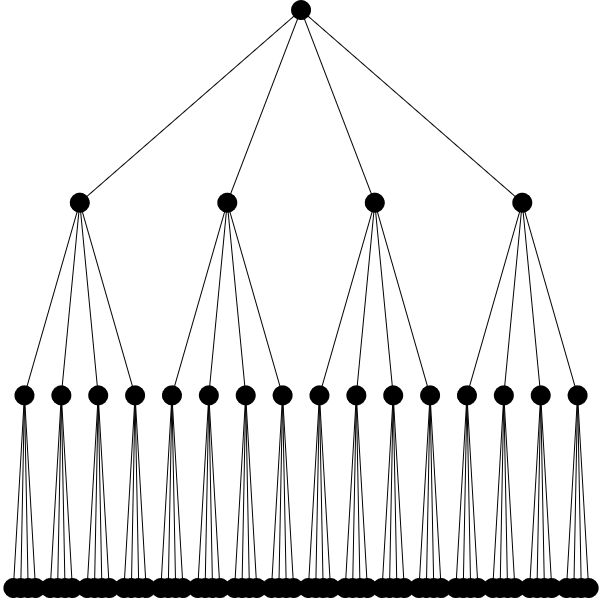
\includegraphics[width=.9\linewidth]{../screenshots/lineargraphexample.PNG}
		\caption{Lineare Baumdarstellung}
		\label{abb:linearbaum}
	\end{minipage}%
	\begin{minipage}{.5\textwidth}
		\centering
		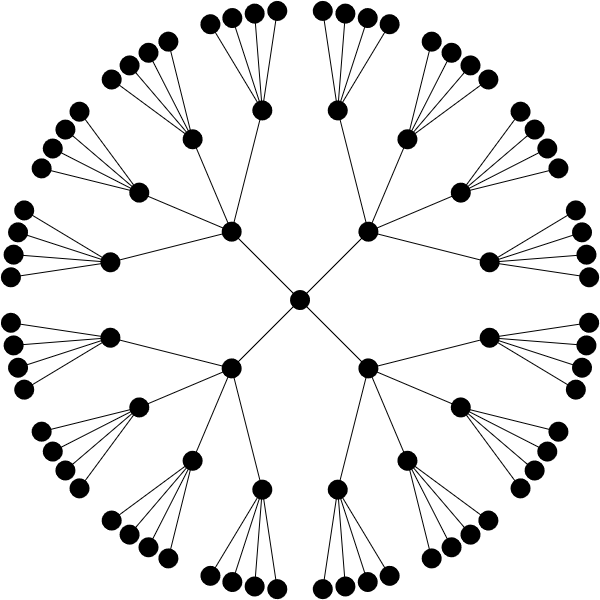
\includegraphics[width=.9\linewidth]{../screenshots/radialgraphexample.PNG}
		\caption{Radiale Baumdarstellung}
		\label{abb:radialbaum}
	\end{minipage}
\end{figure}
Die Abbildungen \ref{abb:linearbaum} und \ref{abb:radialbaum} zeigen einen Vergleich zwischen einem Baum in linearer (Abb. \ref{abb:linearbaum}) und in radialer Anordnung (Abb. \ref{abb:radialbaum}). In beiden Fällen ist derselbe Baum der Höhe 4 auf gleicher Fläche abgebildet. Er besteht aus 105 Knoten, wobei alle inneren Knoten jeweils vier Nachfolger haben. Der Wurzelknoten befindet sich beim linearen Layout am oberen Rand. Die übrigen Knoten sind in drei horizontalen Linien darunter angeordnet, wobei die Kinder der Wurzel auf der obersten Linie liegen, deren Kinder auf der mittleren und deren Kinder auf der untersten Linie. Beim radialen Layout ist die Wurzel in der Mitte abgebildet und alle anderen Knoten in drei konzentrischen Kreisen darum herum. Knoten der Tiefe 1 liegen auf dem innersten Kreis, der Tiefe 2 auf dem mittleren Kreis und die Blätter auf dem äußeren Kreis. Den Mittelpunkt der Kreise bildet die Wurzel. Man sieht deutlich, dass im Fall der vertikalen Anordnung (Abb. \ref{abb:linearbaum}) nicht ausreichend Platz für alle Blätter zur Verfügung steht, wodurch es zu starken Überschneidungen kommt. In der radialen Anordnung (Abb. \ref{abb:radialbaum}) können hingegen alle Knoten überschneidungsfrei dargestellt werden.\\
Um den Grund dafür zu veranschaulichen vergleicht man den Platz, der bei den beiden Herangehensweisen auf einer einzelnen Stufe des Baumes zur Verfügung steht. Unter der Annahme, dass für die gesamte Darstellung ein Quadrat mit Seitenlänge $a$ zur Verfügung steht und alle Knoten einen Durchmesser von 1 haben ergibt sich für den Platz $l_{linear}$ bzw. $l_{radial}$, der auf einer Stufe des Baumes verfügbar ist 
\begin{align*}
&l_{linear} = a\\
&l_{radial} = 2 \cdot \pi \cdot r\mspace{40mu} mit\quad 0\leq r \leq \frac{a}{2} .
\end{align*}
Dabei bezeichnet $r$ den Abstand einer Stufe zum Wurzelknoten. Setzt man $l_{radial}$ und $l_{linear}$ gleich und stellt nach $r$ um, so ergibt sich
\begin{align*}
&l_{linear} = l_{radial}\\
\Rightarrow \mspace{40mu} &a = 2 \cdot \pi \cdot r\\
\Rightarrow \mspace{40mu} &\frac{a}{2 \cdot \pi} = r\\
\Rightarrow \mspace{40mu} &r \approx \frac{a}{6}.
\end{align*}
Da $l_{linear}$ konstant ist kann man daraus ableiten
\begin{align*}
l_{radial} > l_{linear} \mspace{40mu} \Leftrightarrow  \mspace{40mu} r > \frac{a}{6}.
\end{align*}
Das bedeutet, dass ab einem Abstand zur Wurzel von mehr als $\frac{a}{6}$ im radialen Layout mehr Platz für jede Stufe verfügbar ist. Außerdem gilt: Je größer der Abstand $r$, desto mehr Platzersparnis. Das ist vor allem deshalb von Interesse, weil Bäume in der Regel die Eigenschaft haben, dass mit wachsender Baumtiefe auch die Anzahl der Knoten in der jeweiligen Tiefe wächst und diese tiefer liegenden Knoten in der kreisförmigen Darstellung weiter von der Wurzel entfernt sind. Das radiale Layout bietet somit genau dann mehr Platz, wenn üblicherweise mehr Platz benötigt wird.
Aufgrund dieser Erkenntnis und der Tatsache, dass beide Darstellungsformen gute Übersichtlichkeit aufweisen, fiel die Wahl letztendlich auf das radiale Layout.

\subsection{Polarkoordinaten}
D3 bietet zur Berechnung einer sinnvollen Knotenanordnung von Bäumen die Funktion $d3.tree()$ an, welche unter Verwendung des Reingold-Tilford Algorithmus \todo{quelle} allen Knoten eines Baumes x- und y-Koordinaten jeweils im Bereich von 0 bis 1 zuordnet. Es liegt dann in der Hand des Programmierers, diese sinnvoll zu interpretieren. Um die Knoten, wie in Abbildung \ref{abb:radialbaum} gezeigt in konzentrischen Kreisen anzuordnen, eignen sich Polarkoordinaten ausgezeichnet. Einem Vorschlag aus der Dokumentation von D3 folgend \todo{quelle} wird die y-Koordinate als Radius $\rho$, die x-Koordinate als Polarwinkel $\varphi$ in Radiant interpretiert. \todo{bild}
\begin{align*}
&\rho = y\\
&\varphi = 2 \cdot \pi \cdot x
\end{align*}
Zur Darstellung auf dem Bildschirm müssen $\rho$ und $\varphi$ anschließend in kartesische Koordinaten $x_{screen}$ und $y_{screen}$ umgerechnet werden. Die allgemeinen Umrechnungsformeln ergeben sich als
\begin{align*}
&x_{screen} = \rho \cdot \cos (\varphi)\\
&y_{screen} = \rho \cdot \sin (\varphi).
\end{align*}
Bei dieser Umrechnung wird allerdings noch nicht berücksichtigt, dass die gegebenen Polarkoordinaten auf generischen Koordinaten im Bereich $[0,1]$ basieren. Zur korrekten Positionierung müssen noch eine Skalierung auf die verfügbare Breite (width) $w$ und Höhe (height) $h$, sowie eine Verschiebung in die Mitte der Anzeige vorgenommen werden. Es entstehen die endgültigen Formeln:
\begin{align}
&x_{screen} = \rho \cdot \cos (\varphi) \cdot w + \frac{w}{2} \label{eq:polkarthx}\\
&y_{screen} = \rho \cdot \sin (\varphi) \cdot h + \frac{h}{2}.\label{eq:polkarthy}
\end{align}
Da die theoretische Seite des grundlegenden Layouts damit geklärt ist, bleibt noch zu erörtern, wie Knoten in der Praxis ihren Weg auf den Bildschirm finden. Auch hier kommt wieder D3 zum Einsatz.

\section{Anzeigen der Knoten mit D3}

Um mit D3 auf den Bildschirm zu zeichnen gibt es verschiedene Möglichkeiten. In der Regel werden die HTML-Elemente $canvas$ oder $svg$ als Zeichenfläche verwendet. Beide haben Vor- und Nachteile, die vor einer Entscheidung abzuwägen sind.

\subsection{Canvas versus SVG}\label{sec:cvs}
Der größte Unterschied zwischen $canvas$ und $svg$ Elementen besteht darin, dass ein $svg$ jedes Objekt, dass es anzeigen soll einzeln als HTML-Element hinterlegt während ein $canvas$ nur das insgesamt entstehende Bild speichert. Für den Browser bedeutet das, dass bei einem $canvas$ nur die Darstellung eines  einzelnen Bildes zu berechnen ist, während bei einem $svg$ alle dargestellten Objekte getrennt behandelt werden. Das führt dazu, dass mit wachsender Zahl anzuzeigender Elemente die Berechnungsdauer des $svg$ stärker ansteigt, als die des $canvas$. Das einzelne Speichern der Anzeigebausteine bringt aber auch Vorteile mit sich. Es ist einfach ein einzelnes Objekt auf dem Bildschirm zu verändern, indem man dessen $svg$-Attribute anpasst, weil der Browser sich dann selbst um die Aktualisierung der Anzeige kümmert. D3 bietet mit seinen $transitions$ eine simple Möglichkeit beliebige Animationen auf einem $svg$ Element durchzuführen, was auf einem $canvas$ umständlicher mit D3 $interpolators$ und einer Funktion zu lösen ist, die für jedes Einzelbild der Animation das Bild neu zeichnet. Allgemein scheint die Nutzung eines $svg$-Elements zur Darstellung von Daten mit D3 die am häufigsten gewählte Herangehensweise, was zu einer großen Menge Beispiele führt, die zur Inspiration genutzt werden können. Auch in diesem Fall fällt die Wahl darauf D3 in Verbindung mit $svg$ einzusetzen. Diese Entscheidung wird vor allem durch die in Kapitel \ref{sec:reduzieren} beschriebene Reduzierung der angezeigten Knoten untermauert, denn der große Vorteil schnellerer Berechnung auf $canvas$-Elementen fällt damit kaum noch ins Gewicht.

\subsection{Datenstruktur}
Zur Speicherung der Baumdaten werden die Knoten in eine D3 $hierarchy$ Umgewandelt. Es ist zu beachten, dass eine $hierarchy$ nur durch ein einzelnes Objekt repräsentiert wird, welches die Wurzel ($root$) des Baumes darstellt. Um eine Array aller Knoten zu erhalten kann $root.descendants()$ aufgerufen werden. Jeder einzelne Knoten ist dabei ein Javascript-Objekt, das wichtige Informationen, wie id, Name und ausführliche Beschreibung enthält. Wendet man $d3.tree()$ auf die $hierarchy$ an, so kommen zusätzlich noch x- und y-Koordinaten dazu. Unter Einsatz dieser Daten kann der Baum auf ein $svg$-Element gezeichnet werden.

\subsection{Anzeige auf SVG}
Mit Hilfe von $d3.select()$ und $selection.append()$ wählt man zuerst das HTML-Element aus, welches die Anzeige beinhalten soll, und hängt ihm ein $svg$ an. Der Rückgabewert von $append$ ist dabei eine $selection$, die nur das $svg$-Element enthält. Diese nutzt man beim weiteren Vorgehen immer dann, wenn eine Änderung am $svg$ vorgenommen werden soll.\\
Dinge auf einem $svg$ anzuzeigen bedeutet, ihm Unterelemente hinzuzufügen. Es gilt also diese aus den gegebenen Knotendaten zu generieren. Es ergibt Sinn, dem $svg$ mit $append$ zunächst zwei Gruppen ($svg$-Element $g$) für Knoten und Kanten des Baumes einzufügen. Diese werden im Weiteren als Knotengruppe und Kantengruppe bezeichnet. \todo{d3 Vorgehensweise beim Hinzufügen von Elementen im Background erklären (select()/selectAll() -\textgreater\ data() -\textgreater\ enter() -\textgreater\ append()) und das hier dann umschreiben?}
\begin{figure}
	\centering
	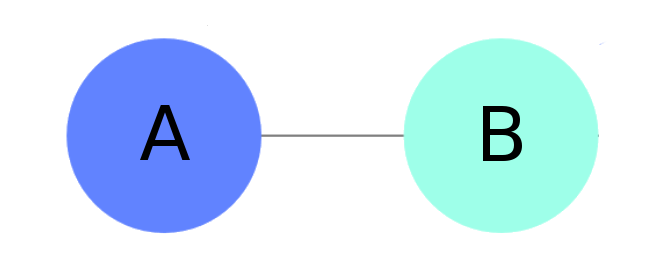
\includegraphics[width=\linewidth]{../screenshots/knotendesign.PNG}
	\caption{Konzept für Knoten und Kanten}
	\label{abb:design}
\end{figure} 
Abbildung \ref{abb:design} zeigt das gewünschte Aussehen für Knoten und Kanten. Zu sehen sind zwei Knoten als Kreise mit Beschriftung A und B. Die Kante zwischen den Beiden Knoten ist dargestellt als Linie, die beide Kreise miteinander verbindet. Die Unterschiedlichen Farben der Knoten zeigen an, dass sie verschiedene Knotentypen haben. Im medizinischen Kontext könnte es sich zum Beispiel um ein Symptom A und eine Diagnose B handeln.\\
Mit $selectAll$ werden alle $g$ Elemente innerhalb der Knotengruppe ausgewählt (zu Beginn gibt es keine) und die entstehende $selection$ wird durch $selection.data()$ mit Daten verknüpft. Als Datensatz dient dabei die von $root.descendants()$ zurückgegebene Liste aller Knoten. $selection.enter()$ liefert dann die Knoten, welche noch kein zugehöriges $g$-Element in der Knotengruppe haben und es wird für jeden ein solches erstellt mit einem $circle$- und $text$-Element im Inneren. Die Vorgehensweise beim einfügen der Kanten verläuft analog, mit dem Unterschied, dass als Datensatz die Rückgabe von $root.links()$ genutzt wird, welche eine Liste aller Kanten des Baumes ist. Anstelle von Gruppenelementen mit $circle$ und $text$ als Inhalt fügt man der Kantengruppe $path$-Elemente ein, die sich mit $d3.line()$ generieren lassen.\\
Mobile Geräte haben keine einheitlichen Bildschirmgrößen. Daher variiert Der Radius der Kreise, die die Knoten repräsentieren. Die Größe der Aufschrift soll so berechnet werden, dass sie so groß wie möglich ist, aber nicht den umgebenden Kreis überschreitet.

\subsection{Berechnen der Schriftgröße}
\todo{aufteilung auf zwei zeilen implementieren}
Angaben von Schriftgrößen beziehen sich auf die Höhe der Buchstaben \todo{quelle}. Das bedeutet nicht notwendigerweise, dass eine Schriftgröße von 10px zu Buchstaben führt, die exakt Zehn Pixel hoch sind, sondern dass die Höhe der Schriftzeichen proportional zur angegebenen Schriftgröße ist. Das bedeutet auch, dass die Breite eines Buchstabens dazu proportional ist, da er beim Vergrößern nicht verzerrt werden soll, wodurch das Verhältnis von Höhe zu Breite immer gleich bleibt. Diese Tatsache lässt sich auf ganze Texte übertragen...

\section{Reduzieren der angezeigten Knoten}\label{sec:reduzieren}
Nachdem mit dem radialen Layout (Kapitel \ref{sec:radial}) eine erste Maßnahme zum Einsparen von Platz ergriffen wurde, stellt sich als nächstes die Frage, wie die Übersichtlichkeit weiter verbessert werden kann. Da Knoten auf dem Bildschirm Informationen in Form von Text beinhalten sollen, ist es abzusehen, dass jeder einzelne Knoten mehr Platz einnehmen wird, als z.B. in Abbildung \ref{abb:radialbaum} gezeigt ist. Es bietet sich an, immer nur aktuell relevante Knoten ein- und irrelevante auszublenden. Das erfordert je nach Eingabe dynamische Änderungen an der Anzeige der Baumstruktur (Kapitel \ref{sec:dynamische_aktual}). Zunächst muss jedoch entschieden werden, welche Knoten aktuell relevant oder irrelevant sind. 
\begin{figure}
	\centering
	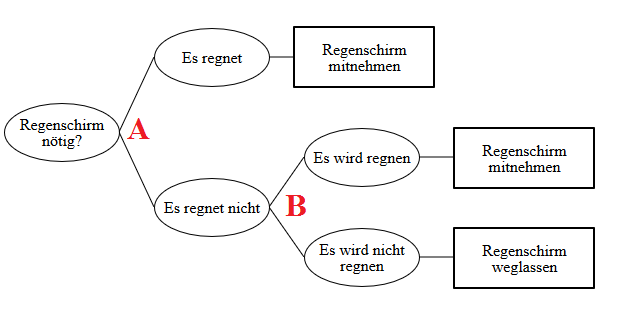
\includegraphics[width=\linewidth]{../screenshots/entscheidungsbaum_bsp.PNG}
	\caption{Ein simpler Entscheidungsbaum}
	\label{abb:entsch_baum_bsp}
\end{figure}
In Abbildung \ref{abb:entsch_baum_bsp} ist beispielhaft ein Entscheidungsbaum zu sehen, der in stark vereinfachter Form die Entscheidungsfindung zur Frage, ob ein Regenschirm nötig ist, zeigt. Innere Knoten sind als Ellipsen dargestellt und Blätter, welche endgültige Ergebnisse repräsentieren, sind rechteckig. Die Beschriftung der Knoten zeigt an, welche Aussage oder Frage sie symbolisieren. Die beiden Stellen, an denen Entscheidungen getroffen werden müssen, sind mit $A$ und $B$ markiert. In Situation $A$ gilt es zu entscheiden, ob es regnet oder nicht. Um diese Entscheidung treffen zu können, ist nicht relevant, ob es zu einem späteren Zeitpunkt regnen wird oder nicht und welche Ergebnisse sich daraus ableiten lassen. Bei $B$ wiederum sind vorherige Entscheidungsmöglichkeiten nicht von Interesse, ebenso wie die Folgen davon, ob es regnen wird oder nicht. Man kann sagen, dass bei jeder Verzweigung nur die zur Verfügung stehenden Alternativen relevant sind und angezeigt werden müssen. Da es jedoch nicht nur darum geht, so viel Platz wie möglich zu sparen, sondern auch darum, eine übersichtliche und intuitiv Verständliche Darstellung zu finden ist es hilfreich, außerdem noch den Knoten, von dem die Verzweigung ausgeht zu zeigen. Bei $A$ also den Knoten \glqq Regenschirm nötig\grqq , bei $B$ \glqq Es regnet nicht\grqq . Auf diese Art ist es leichter die Orientierung zu behalten, selbst wenn ein Großteil des Baumes nicht sichtbar ist.

\section{Navigieren durch den Baum}\label{sec:dynamische_aktual}
Durch das Ausblenden vieler der Knoten muss nun eine Möglichkeit geschaffen werden, von einer Entscheidung zur nächsten zu navigieren, wobei immer wieder irrelevante Knoten aus- und relevant gewordene eingeblendet werden. Das wird möglich gemacht, indem die Baumanzeige auf Berührung hin dynamisch aktualisiert wird. Es gilt dabei, dass der Knoten, von dem die aktuelle Verzweigung ausgeht, in der Mitte des Bildschirms zu sehen ist und die nachfolgenden Entscheidungsmöglichkeiten im Kreis darum herum angeordnet werden.
\begin{figure}
	\centering
	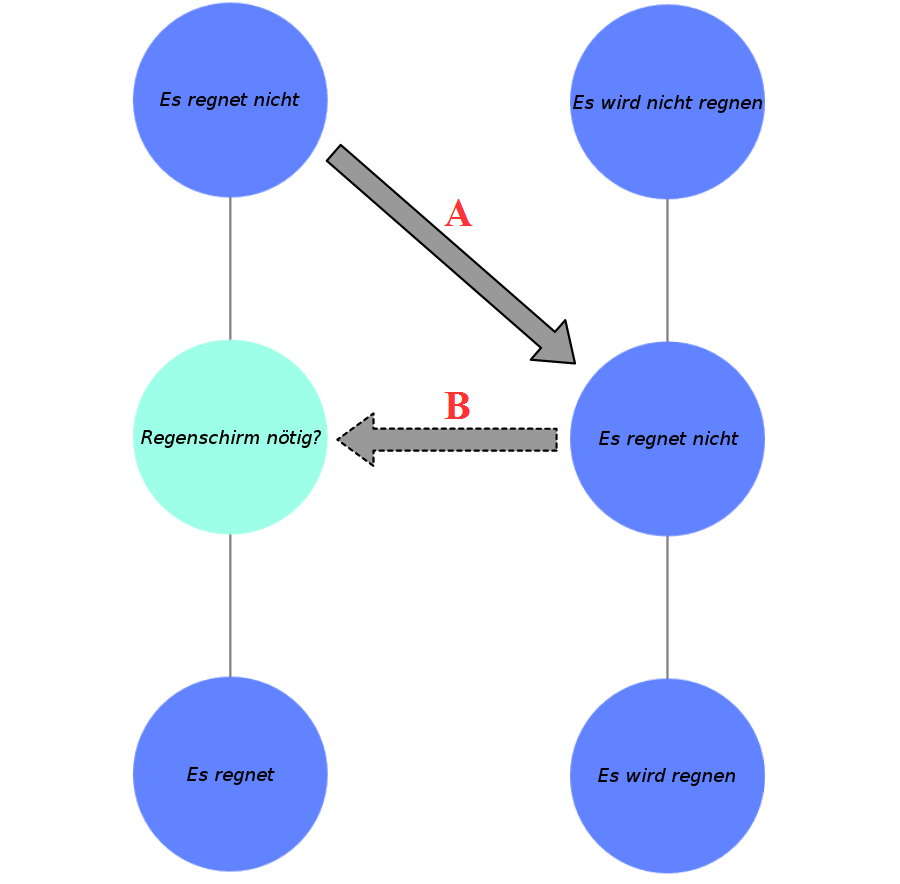
\includegraphics[width=\linewidth]{../screenshots/baumnavigation.PNG}
	\caption{Beispiel zur Baumnavigation}
	\label{abb:baumnavigation}
\end{figure}
Abbildung \ref{abb:baumnavigation} zeigt die Reaktion des Baumes auf verschiedene Nutzereingaben. Auf der linken Seite ist der Ausgangszustand zu sehen und rechts der Nachfolgezustand. Links ist der mittlere Knoten mit \glqq Regenschirm nötig?\grqq\ beschriftet und dessen Nachfolger mit \glqq Es regnet nicht\grqq\ sowie \glqq es regnet\grqq. Rechts sieht man \glqq Es regnet nicht\grqq\ in der Mitte, \glqq Es wird nicht regnen\grqq\ und \glqq Es wird regnen\grqq\ als Folgeknoten. Die mit $A$ und $B$ beschrifteten Pfeile symbolisieren Reaktionen auf Eingaben, die im Folgenden genauer beschrieben werden. \\Durch Antippen eines der äußeren Knoten wird dieser in die Mitte verschoben und es zeigen sich dessen Nachfolger. Tippt man zum Beispiel in Abbildung \ref{abb:baumnavigation} links \glqq Es regnet nicht\grqq\ an, dann wird dieser, wie Pfeil $A$ zeigt, zum mittleren Knoten, die anderen verschwinden und es erscheinen die neuen Nachfolgeknoten. Möchte man einen Schritt zurück machen, kann der Mittelknoten berührt werden und man wird wieder zur links gezeigten Situation geleitet (illustriert durch Pfeil $B$). Es soll dadurch das Gefühl entstehen, dass man sich durch die Baumstruktur bewegt, wobei besonders die gewählten Animationen (Kapitel \ref{sec:animation}) von großer Wichtigkeit sind. Zuerst ist aber zu klären, wie die interne Datenstruktur verwendet werden kann, um dynamische Aktualisierungen zu ermöglichen.
  
\subsection{Dynamische Aktualisierung}

 
\section{Einsatz von Animationen}\label{sec:animation}
Häufig kommen bei der hier beschriebenen interaktiven Visualisierung Animationen zum Einsatz und spielen dabei für diverse Aspekte eine zentrale Rolle. \todo{verweise auf material design guidelines}

\subsection{Verbesserung von Orientierung und Übersichtlichkeit}
Kapitel \ref{sec:reduzieren} beschreibt, wie zum Einsparen von Platz Knoten weggelassen werden können. Ein daraus folgender Nachteil besteht im Orientierungsverlust. Obwohl die Menge an Informationen auf dem Bildschirm sinkt, was die Übersichtlichkeit verbessert, wird es schwerer zu wissen, wo man sich im Baum gerade befindet. Durch passende Animationen beim in Kapitel \ref{sec:dynamische_aktual} beschriebenen dynamischen Aktualisieren des Baumes kann dem Abhilfe geschaffen werden. Es soll dabei durch die Bewegungen auf dem Bildschirm deutlich werden, welche Veränderung eine Eingabe bewirkt. 
\begin{figure}
	\centering
	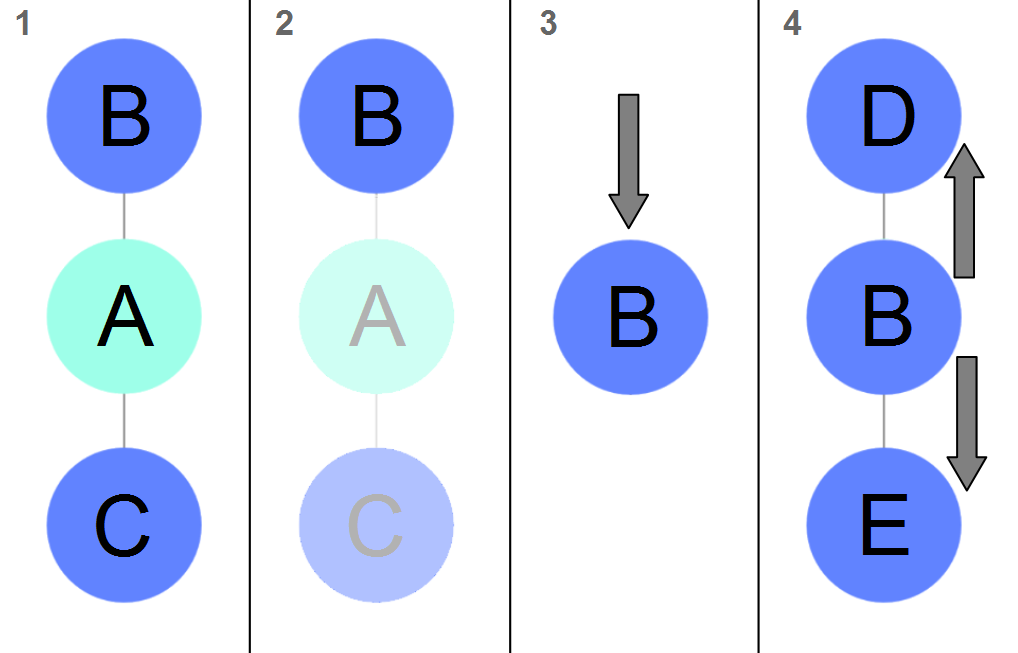
\includegraphics[width=\linewidth]{../screenshots/animation.png}
	\caption{Animation beim Berühren eines Knotens}
	\label{abb:animation}
\end{figure}
Die gewählte Animation beim Navigieren von einem Knoten zum nächsten ist in Abbildung \ref{abb:animation} zu sehen. Von links nach rechts mit 1 bis 4 nummeriert werden die vier wichtigen Zeitpunkte im Bewegungsablauf gezeigt. Situation 1 zeigt den Ausgangszustand: Ein Knoten $A$ mit dessen Nachfolgerknoten $B$ und $C$. Die anderen drei Stadien zeigen was geschieht, wenn man $B$ antippt. Zunächst werden bei 2 die Knoten $A$ und $C$ durchsichtiger, bis sie nicht mehr zu sehen sind. Anschließend bewegt sich $B$ in die Mitte der Anzeige (zu sehen bei 3) und zuletzt bewegen sich zu Zeitpunkt 4 von $B$ aus die Knoten $D$ und $E$ nach außen. \\
Das Ausblenden von $A$ und $C$ verdeutlicht, dass beide nicht mehr relevant sind, geschieht aber zur Vermeidung von Verwirrung nicht von einem Moment auf den anderen. Die Bewegung von $B$ in die Mitte lässt leicht nachverfolgen, dass $B$ zum neuen Verzweigungspunkt wird. Wichtig ist dabei, dass $B$ zu keinem Zeitpunkt vom Bildschirm verschwindet oder umherspringt, wodurch klar ist, dass es sich noch immer um denselben Knoten handelt. Zuletzt verdeutlicht die von $B$ ausgehende Bewegung von $D$ und $E$ nach außen, dass diese die Nachfolger von $B$ sind. Der allgemeine Schwerpunkt liegt darauf, es durch kontinuierliche Bewegungen leichter zu machen, dem Geschehen zu folgen, was zu einem intuitiven Verständnis der Vorgänge auf dem Bildschirm führt.

\subsection{Interaktivität}





























































%\chapter{Results}

Second most important chapter. Verifies the theses defined in the previous chapter. Tries to evaluate and analyze the contribution in qualitative or quantitative terms. Ends with a discussion. Approximately 20 to 30 pages. Can be split into multiple chapters.

%\chapter{State of the Art}
Related work. Present state of research and applied solutions concerning the different aspects relevant to the thesis. Discuss differences and similarities to other solutions to the given tackled problem. Approximately 10 to 15 pages.

%
\chapter{Conclusion}

One page. What have we learned in/through this thesis?

Expected thesis length: 90 pages (+-10\%)

% Back Matter (use input to add appendices, if really needed)

%\newpage
\smallerBegin
\pagenumbering{roman}
\bibliographystyle{gerplain}

\bibliography{all_publications}

\smallerEnd

%% end of document

\end{document}